\chapter{Dataset}
\label{ch:dataset}
This chapter discusses the dataset used in our work.

\section{Overview}
An overview of the dataset can be seen in \autoref{fig:dataset_overview}.

\begin{figure}[h]
    \centering
    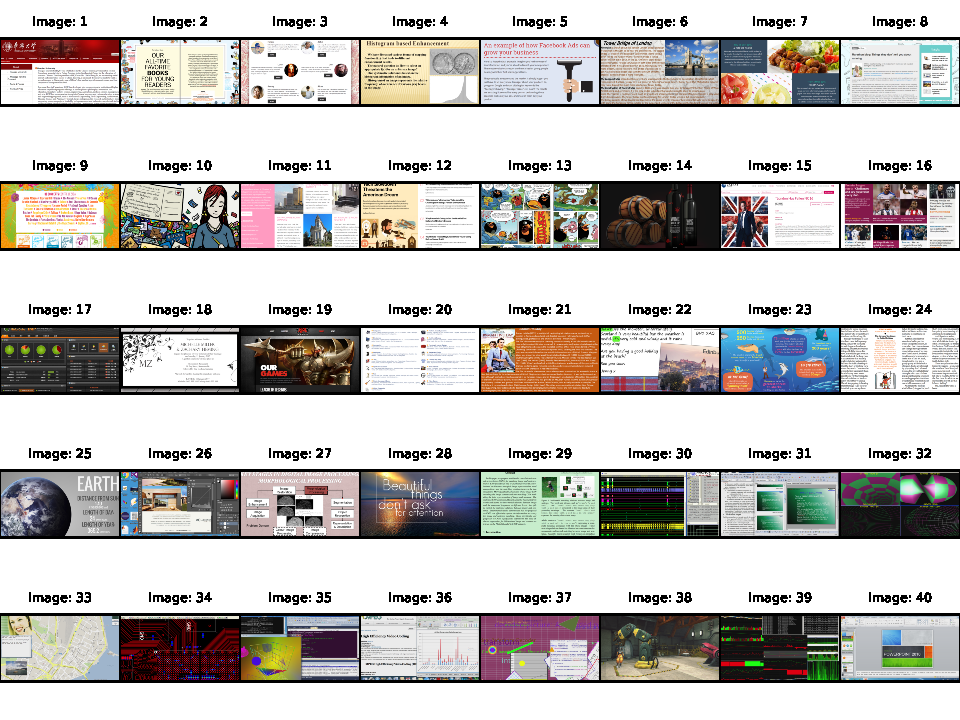
\includegraphics[width=\textwidth]{reference_images}
    \caption{Overview of the dataset.}
    \label{fig:dataset_overview}
\end{figure}


\section{Analysis}

In \autoref{fig:ter_vs_mos} the TER is plotted against the MOS.
It shows the TER and MOS of all 1800 distorted images compared to their reference image.

\begin{figure}[h]
    \centering
    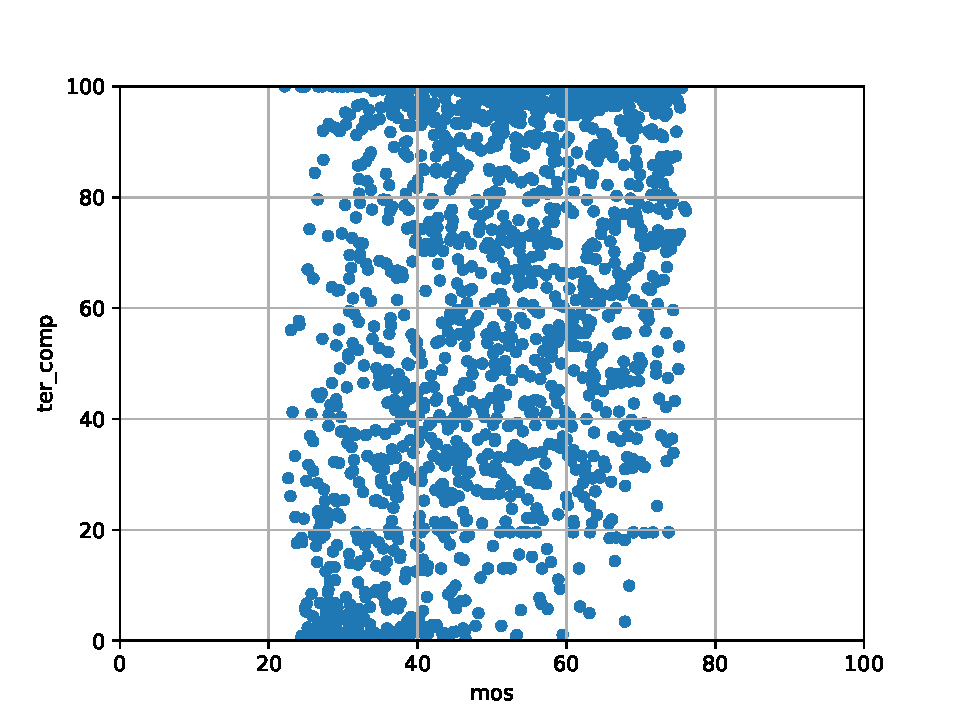
\includegraphics[width=\textwidth]{mosvster_all}
    \caption{TER of all distorted images compared to their reference image plotted against the MOS.}
    \label{fig:ter_vs_mos}
\end{figure}

In \autoref{fig:ter_vs_mos_456} the TER is plotted against the MOS.
We are only using a selection of images in this plot.
These images (SCI4, SCI5, SCI6, SCI22 and SCI29) have their main focus on text, and have simple text structure.
\begin{figure}[h]
    \centering
    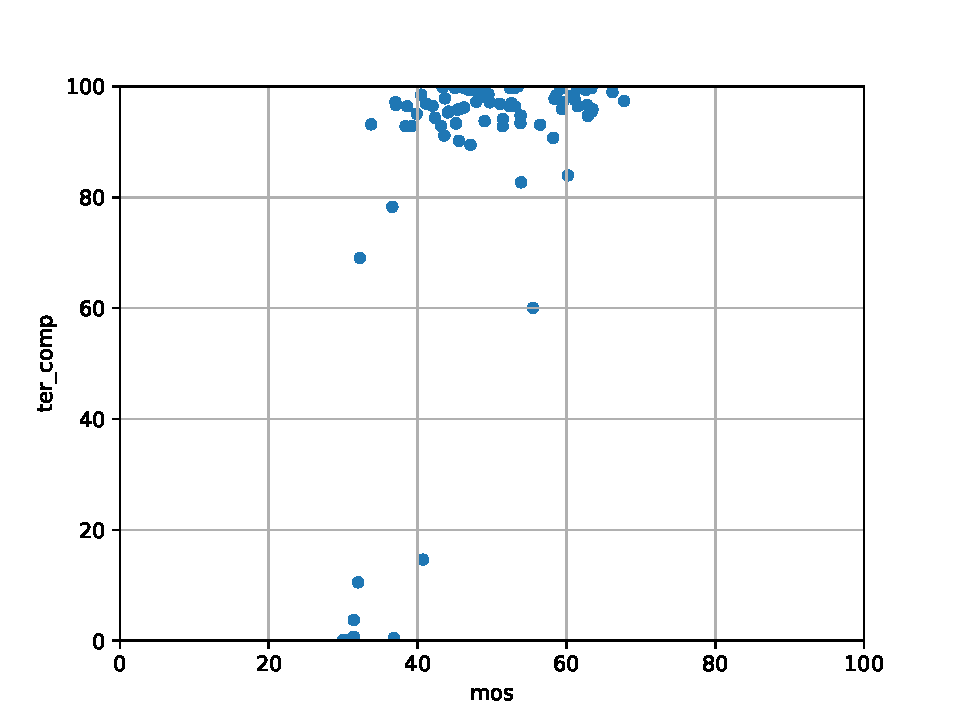
\includegraphics[width=\textwidth]{mosvster__456_22_29__1_4}
    \caption{TER of a selction of distorted images compared to their reference image.}
    \label{fig:ter_vs_mos_456}
\end{figure}
